Bla bla bla ...

This plot shows s-curves with dependencies of Muon Efficiency versus High Voltage Effective (HVeff) for the second version of FEB with PETIROC2B (FEBv1b). Also, this slide showing the mean value of multiplicity for each side. AND efficiency showing without crosstalk impact. Data was taking during GIF++ (ATT=3.3) cosmic tests (September-November 2019). Scintillators placed in the HR of the chamber and covered about ~20cm. This setup includes three protected with leads scintillators inside GIF++ (without outside scintillators)
HR: 500-480=20DACu. (50±10fC)

LR: 500-480=20DACu (50±10fC)

HIGH VOLTAGE EFFECTIVE (X-axis)

Effective HV takes into account the change in pressure and temperature with respect to an HV reference value V0 at given pressure P0 and temperature T0.

\begin{figure}
    % Source: https://twiki.cern.ch/twiki/bin/view/CMSPublic/RPCUpgrade2020#iRPC_tests_Shchablo_Konstantin
    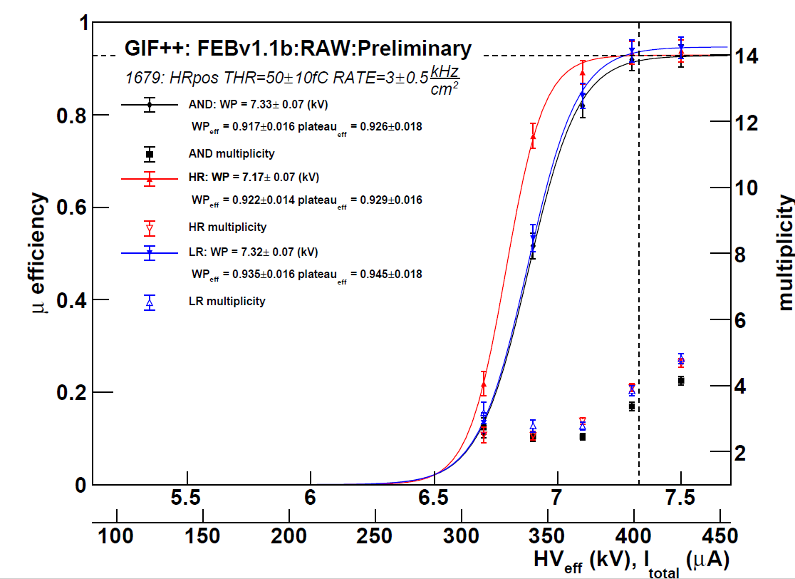
\includegraphics[width=1\textwidth]{uioposter-images/irpc_feb_eff}
    \caption{A capition for iRPC FEB.}
    \label{irpc_feb}
\end{figure}

Bla bla bla ...